% Classic Beamer setup
\documentclass[aspectratio=169]{beamer}
\usetheme{default}
\usecolortheme{default}
\useinnertheme{default}
\useoutertheme{default}

% Grid background
\usepackage{tikz}
\usebackgroundtemplate{
  \tikz[overlay,remember picture]
    \draw[step=0.1cm,gray!30] (current page.south west) grid (current page.north east);
}

% Colors
\definecolor{myaccent}{HTML}{007ACC}
\setbeamercolor{title}{bg=gray!60, fg=black}
\setbeamercolor{frametitle}{bg=gray!60, fg=black}
\setbeamercolor{block title}{bg=black, fg=white}
\setbeamercolor{block body}{bg=white, fg=black}
\setbeamercolor{structure}{fg=black}
\setbeamertemplate{navigation symbols}{}

% Fonts
\usepackage{fontspec}
\usepackage{unicode-math}
\setmainfont[
  Path = fonts/,
  Extension = .ttf,
  UprightFont = UniversRegular,
  BoldFont = UniversBold
]{UniversRegular}
\setsansfont[
  Path = fonts/,
  Extension = .ttf,
  UprightFont = UniversRegular,
  BoldFont = UniversBold
]{UniversRegular}
\setmathfont{Latin Modern Math}
\newfontfamily\thesisserif{Latin Modern Roman}

% Fix \mathcal & \mathfrak
\usepackage{amsmath, amssymb}
\let\mathcal\relax
\DeclareMathAlphabet{\mathcal}{OMS}{cmsy}{m}{n}
\let\mathfrak\relax
\DeclareMathAlphabet{\mathfrak}{U}{euf}{m}{n}

% Extra packages
\usepackage{appendixnumberbeamer}
\usepackage{stmaryrd}
\usepackage{stackengine}
\usepackage{graphicx}
\usepackage{amsthm}
\usepackage{hyperref}
\usepackage{mdframed}

% Title info
\setbeamertemplate{headline}{}
\title{\Huge \textbf{Algebraic Logic of Secrets}}
\author{Made By: \textbf{Omar Gamal Eldin}\\Supervised by: \textbf{Prof. Haythem O. Ismail}}
\institute{}
\date{}

% GUC logo
\addtobeamertemplate{title page}{
  \begin{tikzpicture}[remember picture,overlay]
    \node[anchor=south west,xshift=1.15em,yshift=1.1em] at (current page.south west) {
      
\includegraphics[height=1.4cm]{images/GUC.jpg}
    };
  \end{tikzpicture}
}{}

% Outline bullets
\setbeamertemplate{section in toc}{\textbullet\ \inserttocsection}
\setbeamertemplate{subsection in toc}{\hspace{1.5em}\textbullet~\inserttocsubsection\\}

% Frametitle font size
% === Frametitle font size ===
\setbeamerfont{frametitle}{size=\Huge,series=\bfseries}

\makeatletter
\setbeamertemplate{frametitle}{
  \vskip0.1em
  \begin{beamercolorbox}[wd=\paperwidth,ht=2ex,dp=1ex,leftskip=1em]{frametitle}
    \insertframetitle
  \end{beamercolorbox}
  \vskip0.1em
}
\makeatother

% Custom commands

\newcommand{\nec}{\Box}
\newcommand{\pos}{\Diamond}
\newcommand{\BoxStar}{\fboxsep=1pt\fbox{$\ast$}}

\begin{document}

\frame{\titlepage}

%=========Outline=========%

\begin{frame}
\frametitle{Outline}
% \small
\tableofcontents[hideallsubsections]
\end{frame}

%=========Introduction=========%

\section{Introduction}
\begin{frame}
\frametitle{Introduction}

\begin{columns}[c]
    \column{0.6\textwidth}
    \Large
    \begin{itemize}
        \item AI models and agents are rapidly becoming part of daily life.
        \item They must understand and handle secrets for trust and privacy.
        \item Existing logics do not model secrecy realistically.
    \end{itemize}

    \column{0.4\textwidth}
    \centering
    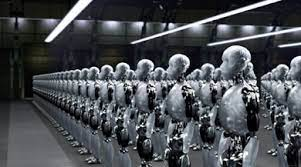
\includegraphics[width=\linewidth]{images/irobot3.png}
\end{columns}

\end{frame}

% \subsection{Secrets}
% \begin{frame}
% \frametitle{What is a Secret?}
% \Large
% \begin{itemize}
%     \item A \textbf{Secret} is a true piece of information that is kept hidden from others.
%     \item Examples:
%     \begin{itemize}
%         \item Classified military maps.
%         \item Personal information like passwords.
%         \item Credit card PINs.
%         \item Hidden treasure locations.
%         % \item Exam questions before release.
%         % \item Corporate trade secrets.
%         % \item Sensitive medical records.
%         % \item Political strategies.
%         % \item Personal relationships (e.g., romantic interests).
%     \end{itemize}
%     \item A Secret is not just the information itself, but rather that it holds a specific confidential meaning.
% \end{itemize}
% \end{frame}

%=========Background=========%

% \section{Background}

% \subsection{Propositional \& Modal Logic}
% \begin{frame}
% \frametitle{Propositional Logic}
%     \Large 
%     \textbf{Propositional Logic (PPL):}
%     \begin{itemize}
%         \item Basic true/false statements combined with connectives.
%         \item No context or agents.
%     \end{itemize}
%     \begin{block}{Example}
%         \[
%         p \wedge q \rightarrow r
%         \]
%     \end{block}
% \end{frame}

% \begin{frame}
% \frametitle{Modal Logic}
%     \Large 
%     \textbf{Propositional Modal Logic (PML):}
%     \begin{itemize}
%         \item Adds modal operators: \\
%         Necessity ($\Box$) and possibility ($\Diamond$).
%         \item Uses possible worlds semantics.
%     \end{itemize}
%     \begin{block}{Example}
%         \[
%         \Box p \rightarrow q, \quad
%         \Diamond r \rightarrow \Box \neg s.
%         \]
%     \end{block}
% \end{frame}

% \begin{frame}
% \frametitle{First-Order Modal Logic (FOML)}
%     \Large 
%     \textbf{First-Order Modal Logic (FOML):}
%     \begin{itemize}
%         \item Extends PML with quantifiers and predicates.
%         \item Allows reasoning about properties of objects.
%     \end{itemize}
%     \begin{block}{Example}
%         \[
%         \forall x (\Box P(x) \rightarrow Q(x)).
%         \]
%     \end{block}
% \end{frame}

% \begin{frame}
% \frametitle{Interpretation of Modal Logic}
% \Large
% \begin{itemize}
%     \item A model $\mathcal{M} = (W, R, A)$ assigns truth to formulas at each world $w \in W$.
% \end{itemize}
% \begin{block}{Basic interpretation rules:}
% \[
% \llbracket T \rrbracket^{\mathcal{M}, w} = \top, 
% \quad 
% \llbracket F \rrbracket^{\mathcal{M}, w} = \bot, 
% \quad 
% \llbracket P \rrbracket^{\mathcal{M}, w} = A(P)(w)
% \]
% \end{block}
% \end{frame}

%=========Theory of Secrets=========%

\section{Theory of Secrets}

\begin{frame}
\frametitle{Theory of Secrets}

\begin{columns}[c]

% ====== Column 1: Text ======
\column{0.7\textwidth}

\Large What is a Secret?

\vspace{1em}

\begin{block}{Definition (Secretum and Secreta):}  
\emph{Secreta} (plural of \emph{secretum}), are the propositions representing confidential information.  
Secrets are not these objects themselves, but relations between \emph{secreta} and other entities (e.g., secret keepers and nescients).
\end{block}

% ====== Column 2: Image ======
\column{0.3\textwidth}

\centering

\includegraphics[width=\linewidth]{images/shield.png}

\end{columns}

\end{frame}

\subsection{Intuitions About Secrects}
\begin{frame}
\frametitle{Intuitions About Secrets}
\begin{itemize}
    \item Secrets are distinct from \textbf{secreta} (the propositions being kept secret).
    \item \textbf{Secreta} are propositions, not physical entities.
    \item Secrets require at least one \textbf{secret keeper}.
    \item Secrets require at least one \textbf{nescient} (someone kept unaware).
    \item Keepers and nescients form structured groups, which can change over time.
    \item A secret exists only under a valid \textbf{secrecy condition}.
    \item Secrets are inherently \textbf{temporary}, they expire or get revealed.
    \item Secret keepers \textbf{believe} the secreta and the condition.
    \item Secret keepers do \textbf{not believe} it has been revealed.
    \item Secret keepers \textbf{intend} to prevent revelation while the condition holds.
\end{itemize}
\end{frame}

\subsection{Formal Structure of Secrets}
\begin{frame}
\frametitle{Formal Structure of Secrets}
{\Large
\begin{itemize}
    \item Key components:
    \begin{itemize}
        \Large 
        \item Secretum ($\phi$): the confidential proposition.
        \item Secret Keepers (K): agents maintaining secrecy.
        \item Nescients (N): agents from whom the secret is hidden.
        \item Secrecy Condition ($\psi$): governs how long secrecy holds.
        \item Time (t): when secrecy is evaluated.
    \end{itemize}
\end{itemize}
}
{\normalsize
\begin{block}{Notation:}
\[
Secret(\phi, K, N, \psi, t)
\]
\end{block}
}
\end{frame}

\begin{frame}
\frametitle{Logical Representation}
\begin{itemize}
    \item Secrecy modeled using FOML with quantification and time.
\end{itemize}
\begin{block}{Core operators:}
\[ 
B(A, \phi), \quad I(A, \phi), \quad R(A, \phi), \quad H(\phi, t), \quad Mem(A, G), \quad \BoxStar \phi 
\]
\normalsize where:
\begin{itemize}
    \item $B(A, \phi)$: Agent A believes $\phi$.
    \item $I(A, \phi)$: Agent A intends to keep $\phi$ secret.
    \item $R(A, \phi)$: Agent A reveals $\phi$.
    \item $H(\phi, t)$: Holds at time $t$.
    \item $Mem(A, G)$: Agent A is a member of group G.
    \item $\BoxStar \phi$: Represents necessity across histories that share the same past.
\end{itemize}
\end{block}
\end{frame}

\subsection{Types of Secrets}
\begin{frame}
\frametitle{Types of Secrets}
\Large
\begin{itemize}
    \item $Secret_0$: basic secrecy (keepers believe, intend, and do not believe it's revealed).
    \item Stronger types:
    \begin{itemize}
        \Large
        \item $S_1$: $\phi$ not actually revealed.
        \item $S_2$: keepers know they keep it.
        \item $S_3$: keepers believe it hasn't been revealed.
        \item $S_4$: keepers know other keepers.
        \item $S_5$: keepers believe all co-keepers know secrecy.
    \end{itemize}
    \item Real secrets often satisfy multiple types.
\end{itemize}
\end{frame}

\subsection{Modeling Time with VEL}
\begin{frame}
\frametitle{Modeling Time with VEL}

\begin{columns}[c]

\column{0.6\textwidth}

\Large
\begin{itemize}
    \item Versatile Event Logic (VEL) structures time as branching histories.
    \item Each moment (state) has:
    \begin{itemize}
        \item Unique past (history)
        \item Multiple possible futures (branches)
    \end{itemize}
    \item Secrets persist unless an event changes them.
\end{itemize}

\column{0.4\textwidth}

\centering

\includegraphics[width=\linewidth]{images/timeline.png}

\end{columns}

\end{frame}
%=========Algebraic Logic Foundations=========%

\section{Algebraic Logic Foundations}

\subsection{Modal vs Algebraic Logic}
\begin{frame}
\frametitle{Modal vs Algebraic Logic}

\begin{columns}[c]

\column{0.6\textwidth}

\Large
\begin{itemize}
    \item \textbf{Modal Logic:} Possible worlds semantics.
    \item \textbf{Algebraic Logic:} Explicit algebraic structures.
    \item More transparent reasoning steps.
    \item Avoids paradoxes (e.g., self-reference).
    \item Better suited for explainable agent models.
\end{itemize}

\column{0.4\textwidth}

\centering

\includegraphics[width=\linewidth]{images/worlds.png}

\end{columns}

\end{frame}

\subsection{Algebraic Logic of Belief ($Log_AB$)}
\begin{frame}
\frametitle{Algebraic Logic of Belief ($Log_AB$)}
\Large
\begin{itemize}
    \item Avoids possible-world semantics by using Boolean algebra.
\end{itemize}
\begin{block}{Belief function:}
\[
B(a, p)
\]
\normalsize where:
\begin{itemize}
    \item $B(a, p)$: agent $a$ believes proposition $p$.
\end{itemize}
\end{block}
\end{frame}

\begin{frame}
\frametitle{Properties of $Log_AB$}
\centering
{\small
\renewcommand{\arraystretch}{1.5}
\begin{tabular}{|p{4cm}|p{9.5cm}|}
    \hline
    \textbf{Property} & \textbf{$Log_AB$ Term} \\
    \hline
    Meet-distributivity & $\forall a, p_1, p_2\,[B(a, p_1) \wedge B(a, p_2) \Leftrightarrow B(a, p_1 \wedge p_2)]$ \\
    \hline
    Join-distributivity & $\forall a, p_1, p_2\,[B(a, p_1) \vee B(a, p_2) \Leftrightarrow B(a, p_1 \vee p_2)]$ \\
    \hline
    Conceit & $\forall a, p\,[B(a, p) \Rightarrow p]$ \\
    \hline
    Consistency & $\forall a, p\,[B(a, \neg p) \Rightarrow \neg B(a, p)]$ \\
    \hline
    Autoepistemology & $\forall a, p\,[\neg B(a, p) \Rightarrow B(a, \neg p)]$ \\
    \hline
    Positive introspection & $\forall a, p\,[B(a, p) \Rightarrow B(a, B(a, p))]$ \\
    \hline
    Negative introspection & $\forall a, p\,[\neg B(a, p) \Rightarrow B(a, \neg B(a, p))]$ \\
    \hline
    Positive faithfulness & $\forall a, p\,[B(a, B(a, p)) \Rightarrow B(a, p)]$ \\
    \hline
    Negative faithfulness & $\forall a, p\,[B(a, \neg B(a, p)) \Rightarrow \neg B(a, p)]$ \\
    \hline
\end{tabular}
}
\end{frame}

\subsection{Algebraic Logic of States ($Log_AS$)}
\begin{frame}
\frametitle{Algebraic Logic of States ($Log_AS$)}
\Large 
\begin{itemize}
    \item States are terms in a Boolean algebra.
\end{itemize}
\begin{block}{Holding and Time Ordering functions:}
\[
HoldsAt(s, t), \quad t_1 \prec t_2
\]
\normalsize where:
\begin{itemize}
    \item $HoldsAt(s, t)$: state $s$ holds at time $t$.
    \item $t_1 \prec t_2$: time $t_1$ precedes $t_2$.
\end{itemize}
\end{block}
\end{frame}

\subsection{State Classifications in $Log_AS$}
\begin{frame}
\frametitle{State Classifications in $Log_AS$}
\Large
\begin{itemize}
    \item States are classified by temporal stability:
    \begin{itemize}
        \Large 
        \item \textbf{ETER (Eternal)}: is the same at all times.
        \item \textbf{ATEMP (Atemporal)}: unchanged, doesn't depend on time.
        \item \textbf{PERM (Permanent)}: once holds, never stops holding.
        \item \textbf{CO-PERM (Co-Permanent)}: an event's occurrence being in the future.
        \item \textbf{TEMP (Temporary)}: may change over time.
        \item \textbf{TRANS (Transient)}: stops and starts holding over time.
    \end{itemize}
\end{itemize}
\end{frame}

%=========Algebraic Logic of Secrets=========%

\section{Algebraic Logic of Secrets ($Log_ASec$)}

\subsection{Language: Syntax and Semantics}
\begin{frame}
\frametitle{$Log_ASec$: Language}
\begin{itemize}
    \item Combines $Log_AB$, $Log_AS$, and VEL into one framework to model secrets.
    \item Sorts:
    \begin{itemize}
        \item Propositions ($\sigma_P$) (atemporal states)
        \item Agents ($\sigma_A$) $\subseteq$ Individuals ($\sigma_I$)
        \item Groups ($\sigma_G$)
        \item Time ($\sigma_T$)
        \item States ($\sigma_S$)
    \end{itemize}
\end{itemize}
\begin{block}{Functions:}
\[
B(a, p), \; I(a, p), \; R(a, p), \;
Mem(a, G), \; HoldsAt(p, t), \; t_1 \prec t_2, \; \BoxStar \; p
\]
\end{block}
\end{frame}

\subsection{Axioms, Theorems, and Proofs}
\begin{frame}
\frametitle{Axioms}
\Large 
\begin{itemize}
    \item Belief follows KD45:
    \begin{itemize}
        \Large 
        \item Distribution, consistency, positive introspection, and negative introspection.
    \end{itemize}
\end{itemize}
\begin{block}{Belief Axioms:}
    \Large
    \normalfont
    (B1) $B(a, p) \wedge B(a, p \rightarrow q) \rightarrow B(a, q)$ \\
    (B2) $B(a, p) \rightarrow \neg B(a, \neg p)$ \\
    (B3) $B(a, p) \rightarrow B(a, B(a, p))$ \\
    (B4) $\neg B(a, p) \rightarrow B(a, \neg B(a, p))$ \\    
    (B5) $\text{If } \vdash p \text{ then } B(a, p)$
\end{block}
\end{frame}

\begin{frame}
\frametitle{Axioms}
\Large 
\begin{itemize}
    \item Intention follows KD:
    \begin{itemize}
        \Large 
        \item Distribution, consistency.
    \end{itemize}
\end{itemize}
\begin{block}{Intention Axioms:}
    \Large
    \normalfont
    (I1) $I(a, p) \wedge I(a, p \rightarrow q) \rightarrow I(a, q)$ \\
    (I2) $I(a, p) \rightarrow \neg I(a, \neg p)$ \\
    (I3) \text{If } $\vdash p$ \text{ then } $I(a, p)$
\end{block}
\end{frame}

% \begin{frame}
% \frametitle{Axioms}
% \begin{block}{Belief--Intention Bridge Axioms:}
%     \Large
%     \normalfont
%     (IB1) $\neg I(a, p) \rightarrow B(a, \neg I(a, p))$ \\
%     (IB2) $B(a, \neg I(a, p)) \rightarrow \neg I(a, p)$ \\
%     (IB3) $I(a, p) \rightarrow B(a, I(a,  p))$ \\
%     (IB4) $B(a, I(a, p)) \rightarrow I(a, p)$ \\
%     (IB5) $I(a, p) \rightarrow \neg B(a, \neg p)$
% \end{block}
% \begin{block}{Revelation Axioms:}
%     \Large
%     \normalfont
%     (R1) $\text{If } \vdash p \text{ then } R(a, p)$ \\
%     (R2) $\text{If } \vdash p \text{ then } \neg R(a, \neg p)$ \\
%     (R3) $\text{If } \vdash p \rightarrow q \text{ then } R(a, p) \rightarrow R(a, q)$ \\
%     (R4) $R(a, \exists b(R(b, p))) \rightarrow R(a, p)$
% \end{block}
% \end{frame}

% \begin{frame}
% \frametitle{Axioms}
% \begin{block}{Belief--Revelation Bridge Axioms:}
%     \Large
%     \normalfont
%     (BR1) $[B(a, p \rightarrow q) \wedge \neg B(a, \neg p)] \rightarrow [R(a, p) \rightarrow R(a, q)]$ \\
%     (BR2) $R(a, p) \rightarrow B(a, R(a, p))$
% \end{block}
% \begin{block}{Group Membership Axioms:}
%     \Large
%     \normalfont
%     (G1) $Mem(a, [b]) \leftrightarrow (a = b)$ \\
%     (G2) $Mem(a, G_1 \sqcup G_2) \leftrightarrow Mem(a, G_1) \vee Mem(a, G_2)$ \\
%     (G3) $Mem(a, G_1 \sqcap G_2) \leftrightarrow Mem(a, G_1) \wedge Mem(a, G_2)$
% \end{block}
% \end{frame}

\begin{frame}
\frametitle{Theorems}
\begin{itemize}
    \item These theorems can be derived from the axioms:
\end{itemize}
\begin{block}{Theorems:}
    \Large
    \normalfont
    (T1) $R(a, p \wedge q) \rightarrow R(a, p) \wedge R(a, q)$ \\
    (T2) $B(a, p) \rightarrow R(a, p)$ \\
    (T3) $R(a, p) \leftrightarrow R(a, R(a, p))$ \\
    (T4) $B(a, p) \rightarrow B(a, R(a, p))$ \\
    (T5) $B(a, R(a, p)) \rightarrow R(a, p)$ \\
    (T6) $B(a, \neg R(a, p)) \rightarrow \neg R(a, p)$ \\
    (T7) $R(a, B(a, p)) \rightarrow B(a, R(a, p))$
\end{block}
\end{frame}

\subsection{Removing Logical Omniscience}
\begin{frame}
\frametitle{Removing Logical Omniscience}
\Large 
\begin{itemize}
    \item Logical omniscience is undesirable in agent models. In order to avoid it, we drop the K axiom:
    \begin{block}{K Axiom:}
    \[
    B(a, p) \wedge B(a, p \rightarrow q) \rightarrow B(a, q)
    \]
    \end{block}
    \begin{block}{Result:}
        Theorems 4 fails: 
        \[
        B(a, p) \rightarrow B(a, R(a, p))
        \]
    \end{block}
\end{itemize}
\end{frame}

%=========Example=========%

\begin{frame}
\frametitle{Example: Secret in a Group}

\begin{columns}[c]

\column{0.75\textwidth}



\Large
\begin{itemize}
    \item Scenario:
    \begin{itemize}
        \item Agents $x$, $y$, and $z$.
        \item Secret $\phi$ known by $x$ and $y$.
        \item $z$ must not know $\phi$.
    \end{itemize}
    \item Formalization:
    \[
    Secret(\phi, \{x,y\}, \{z\}, \psi, t)
    \]
    \item Secrecy condition $\psi$: Holds until $x$ or $y$ reveals $\phi$.
\end{itemize}

\column{0.25\textwidth}

\centering
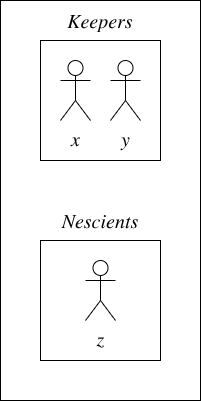
\includegraphics[width=\linewidth]{images/s1.png}

\end{columns}

\end{frame}

\begin{frame}
\frametitle{How $Log_ASec$ Models It}
\begin{itemize}
    \Large 
    \item Belief:
    \[
    B(x, \phi), \; B(y, \phi), \; \neg B(C, \phi)
    \]
    \item Intention:
    \[
    I(x, \neg R(z, \phi)), \; I(y, \neg R(z, \phi))
    \]
    \item Membership:
    \[
    Mem(x, K), \; Mem(y, K), \; Mem(z, N)
    \]
    \item Temporal:
    \[
    HoldsAt(\phi, t), \; HoldsAt(\psi, t)
    \]
\end{itemize}
\end{frame}

\begin{frame}
\frametitle{Secrecy Evolution}

\begin{columns}[c]

\column{0.65\textwidth}

\Large
\begin{itemize}
    \item If $x$ reveals $\phi$ to $z$ at $(h,t)$:
    \begin{itemize}
        \item $R(z, \phi)$ holds at $(h,t)$.
        \item Secrecy condition $\psi$ no longer holds at $(h,t)$.
    \end{itemize}
    \item $Log_{ASec}$ tracks this via:
    \[
    \llbracket R(z, \phi) \rrbracket^{h,t} = \text{true}
    \Longrightarrow 
    \llbracket \psi \rrbracket^{h,t} = \text{false}
    \]
\end{itemize}

\column{0.35\textwidth}

\centering
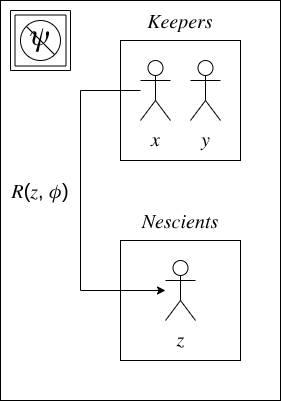
\includegraphics[width=\linewidth]{images/s2.png}

\end{columns}

\end{frame}

%=========Conclusion & Future Work=========%

\section{Conclusion and Future Work}

\subsection{Key Contributions}
\begin{frame}
\frametitle{Key Contributions}
\begin{itemize}
    \Large
    \item Developed a new algebraic logic for secrecy ($Log_ASec$).
    \item Integrated belief, states, Versatile Event Logic, and secrecy conditions.
    \item Defined syntax, semantics, and axioms for core operators.
    \item Removed logical omniscience (K axiom) for realistic agent modeling.
    \item Provided formal proofs for key theorems.
\end{itemize}
\end{frame}

\subsection{Future Directions}
\begin{frame}
\frametitle{Future Directions}
\begin{itemize}
    \Large
    \item Complete proofs for all theorems not covered.
    \item Could be implemented in Prolog for automated secrecy reasoning.
    \item Simulate agent reasoning in secrecy scenarios.
    \item Apply to real-world privacy and information security use cases.
    \item Further refinement of axioms and theorems.
\end{itemize}
\end{frame}

%=========References=========%

% \begin{frame}
% \frametitle{References}
% \footnotesize
% \begin{itemize}
%     \item [1] Brandon Bennett and Antony P. Galton. A unifying semantics for time and events.
%     Artificial Intelligence, 153(1):13–48, 2004. Logical Formalizations and Commonsense
%     Reasoning.
%     \item [2] Patrick Blackburn, Maarten de Rijke, and Yde Venema. Modal Logic. Cambridge
%     University Press, 2001.
%     \item [3] Thomas Bolander. Self-Reference and Paradox. In Edward N. Zalta and Uri Nodel-
%     man, editors, The Stanford Encyclopedia of Philosophy. Metaphysics Research Lab,
%     Stanford University, Fall 2024 edition, 2024.
%     \item [4] Ronald Fagin, Joseph Y. Halpern, Yoram Moses, and Moshe Y. Vardi. Reasoning
%     About Knowledge. MIT Press, 1995.
%     \item [5] James Garson. Modal Logic. In Edward N. Zalta and Uri Nodelman, editors, The
%     Stanford Encyclopedia of Philosophy. Metaphysics Research Lab, Stanford Univer-
%     sity, Spring 2024 edition, 2024.
%     \item [6] Paul R. Halmos. The basic concepts of algebraic logic. Journal of Symbolic Logic,
%     23(2):223–223, 1958.
%     \item [7] Joseph Y. Halpern and Kevin R. O’Neill. On the logic of secrecy. Journal of Com-
%     puter Security, 12(2):229–272, 2004.
% \end{itemize}
% \end{frame}

% \begin{frame}
% \frametitle{References (cont.)}
% \footnotesize
% \begin{itemize}
%     \item [8] Peter Hawke, Aybuke Ozgun, and Francesco Berto. The fundamental problem of
%     logical omniscience. Journal of Philosophical Logic, 49(4):727–766, 2020.
%     \item [9] Haythem O. Ismail. $Log_AB$: A first-order, non-paradoxical, algebraic logic of belief.
%     Logic Journal of the IGPL, 20(5):774–795, 03 2012.
%     \item [10] Haythem O. Ismail. Stability in a commonsense ontology of states. Proceedings of
%     the Eleventh International Symposium on Logical Formalization of Commonsense
%     Reasoning (COMMONSENSE 2013), Agya Napa, Cyprus, 2013.
%     \item [11] Haythem O. Ismail and Merna Shafie. A commonsense theory of secrets. IOS Press,
%     Formal Ontology in Information Systems:77–91, 2020.
%     \item [12] Robert Kowalski and Marek Sergot. A logic-based calculus of events. New Generation
%     Computing, 4(1):67–95, 1986.
%     \item [13] John-Jules Meyer and Wiebe van der Hoek. Epistemic Logic for AI and Computer
%     Science. Cambridge University Press, 2004.
% \end{itemize}
% \end{frame}
  
%=========End=========%

\begin{frame}[c]
\centering
\Huge
\textbf{Thank you!}

\vspace{1cm}

\LARGE
Questions?
\end{frame}

%========= =========%

\end{document}